\documentclass[11pt]{article}
% Shared preamble of the RMC kernel write-ups (% Shared preamble of the RMC kernel write-ups (% Shared preamble of the RMC kernel write-ups (\input{preamble} after \documentclass).
\usepackage[margin=1in]{geometry}
\usepackage{amsmath,amssymb,bm}
\usepackage{graphicx}
\usepackage{booktabs}
\usepackage{hyperref}

\newcommand{\dd}{\,\mathrm{d}}
\newcommand{\Ein}{E}
\newcommand{\Eout}{E'}
\newcommand{\Ecm}{E_{c}}
\newcommand{\mucm}{\mu_{c}}
\newcommand{\mulab}{\mu_0}

% Common closing section: how the verification figures are produced
\newcommand{\verificationmethod}{%
Each figure is produced by \texttt{verification/verify\_laws.py}. For an incident
energy $\Ein$ along $+z$, $10^6$ collisions are sampled with MC/DC's own reaction
sampler (\texttt{sample\_elastic\_scattering}, \texttt{sample\_inelastic\_scattering}
or \texttt{sample\_fission}), and every emitted neutron is histogrammed in
$48 \times 24$ bins of $(\Eout, \mulab)$, with $\mulab$ the lab cosine to $+z$. The
inverted kernel used by RMC is integrated over the same bins (Gauss--Legendre panels;
two-body lines are split where $\mulab^*(\Eout)$ crosses a cosine edge), multiplied by
the number of collisions, and compared with a $\chi^2$ test over bins with at least 5
expected counts (the rest pooled into one bin). The tables list $\chi^2/\mathrm{dof}$,
its $p$-value, the emitted neutrons per collision (sampled vs.\ the integral of the
inverted kernel), and the largest relative change of a bin integral when the
quadrature panels are doubled. Left panels: outgoing-energy marginal; middle:
lab-cosine marginal; right: per-bin $z = (\text{sampled} - \text{inverted}) /
\sqrt{\text{inverted}}$.}
 after \documentclass).
\usepackage[margin=1in]{geometry}
\usepackage{amsmath,amssymb,bm}
\usepackage{graphicx}
\usepackage{booktabs}
\usepackage{hyperref}

\newcommand{\dd}{\,\mathrm{d}}
\newcommand{\Ein}{E}
\newcommand{\Eout}{E'}
\newcommand{\Ecm}{E_{c}}
\newcommand{\mucm}{\mu_{c}}
\newcommand{\mulab}{\mu_0}

% Common closing section: how the verification figures are produced
\newcommand{\verificationmethod}{%
Each figure is produced by \texttt{verification/verify\_laws.py}. For an incident
energy $\Ein$ along $+z$, $10^6$ collisions are sampled with MC/DC's own reaction
sampler (\texttt{sample\_elastic\_scattering}, \texttt{sample\_inelastic\_scattering}
or \texttt{sample\_fission}), and every emitted neutron is histogrammed in
$48 \times 24$ bins of $(\Eout, \mulab)$, with $\mulab$ the lab cosine to $+z$. The
inverted kernel used by RMC is integrated over the same bins (Gauss--Legendre panels;
two-body lines are split where $\mulab^*(\Eout)$ crosses a cosine edge), multiplied by
the number of collisions, and compared with a $\chi^2$ test over bins with at least 5
expected counts (the rest pooled into one bin). The tables list $\chi^2/\mathrm{dof}$,
its $p$-value, the emitted neutrons per collision (sampled vs.\ the integral of the
inverted kernel), and the largest relative change of a bin integral when the
quadrature panels are doubled. Left panels: outgoing-energy marginal; middle:
lab-cosine marginal; right: per-bin $z = (\text{sampled} - \text{inverted}) /
\sqrt{\text{inverted}}$.}
 after \documentclass).
\usepackage[margin=1in]{geometry}
\usepackage{amsmath,amssymb,bm}
\usepackage{graphicx}
\usepackage{booktabs}
\usepackage{hyperref}

\newcommand{\dd}{\,\mathrm{d}}
\newcommand{\Ein}{E}
\newcommand{\Eout}{E'}
\newcommand{\Ecm}{E_{c}}
\newcommand{\mucm}{\mu_{c}}
\newcommand{\mulab}{\mu_0}

% Common closing section: how the verification figures are produced
\newcommand{\verificationmethod}{%
Each figure is produced by \texttt{verification/verify\_laws.py}. For an incident
energy $\Ein$ along $+z$, $10^6$ collisions are sampled with MC/DC's own reaction
sampler (\texttt{sample\_elastic\_scattering}, \texttt{sample\_inelastic\_scattering}
or \texttt{sample\_fission}), and every emitted neutron is histogrammed in
$48 \times 24$ bins of $(\Eout, \mulab)$, with $\mulab$ the lab cosine to $+z$. The
inverted kernel used by RMC is integrated over the same bins (Gauss--Legendre panels;
two-body lines are split where $\mulab^*(\Eout)$ crosses a cosine edge), multiplied by
the number of collisions, and compared with a $\chi^2$ test over bins with at least 5
expected counts (the rest pooled into one bin). The tables list $\chi^2/\mathrm{dof}$,
its $p$-value, the emitted neutrons per collision (sampled vs.\ the integral of the
inverted kernel), and the largest relative change of a bin integral when the
quadrature panels are doubled. Left panels: outgoing-energy marginal; middle:
lab-cosine marginal; right: per-bin $z = (\text{sampled} - \text{inverted}) /
\sqrt{\text{inverted}}$.}


\title{Inverted kernel: elastic scattering, target at rest}
\date{}

\begin{document}
\maketitle

\noindent Applies above the free-gas threshold, $\Ein > 400\,kT$ (below it see
\texttt{free\_gas.tex}). Code: \texttt{delta\_lab\_line} in
\texttt{mcdc/rmc/reaction.py}, \texttt{elastic\_*} in \texttt{mcdc/rmc/kinematics.py}.

\section{What MC/DC samples}

\texttt{sample\_elastic\_scattering} (target at rest):
\begin{enumerate}
  \item $\mucm$ from the elastic angular distribution, a multi-table distribution read
  \emph{without} unit-base scaling: with incident grid $E_i \le \Ein < E_{i+1}$ and
  $f = (\Ein - E_i)/(E_{i+1} - E_i)$, table $i$ is used with probability $1-f$ and
  table $i+1$ with probability $f$ (off the grid: the edge table);
  \item the neutron speed $v$ from $\Ein$ with the relativistic relation
  $v = c\sqrt{\Ein(\Ein + 2m)}/(\Ein + m)$, the COM velocity $\bm v/(1+A)$, rotation
  by $\mucm$ in the COM frame, and back to the lab;
  \item the outgoing energy from the lab speed by the inverse relativistic relation.
\end{enumerate}

\section{Inverted kernel}

\noindent Source for the elastic angular-data representation:
\endfspec{MF=4, Sec.~4.4.1}; \acespec{4.3.9}. The following inversion is derived
from MC/DC's sampler. Its classical velocity addition combined with relativistic
speed conversion is not a fully relativistic two-body collision model.

With $\bm w = A\bm v/(1+A)$ the COM neutron velocity, the lab speed after scattering by
$\mucm$ is
\begin{equation}
  v'^2 = v^2\,\frac{1 + A^2 + 2A\mucm}{(1+A)^2},\qquad
  \mulab = \frac{1 + A\mucm}{\sqrt{1 + A^2 + 2A\mucm}},
\end{equation}
and $\Eout = m(\gamma' - 1)$, $\gamma' = (1 - v'^2/c^2)^{-1/2}$. Inverting at a given
$\Eout$:
\begin{equation}
  \mucm^*(\Eout) = \frac{(1+A)^2\, v'^2(\Eout)/v^2 - 1 - A^2}{2A},\qquad
  \left|\frac{\dd\mucm}{\dd\Eout}\right| = \frac{(1+A)^2}{2A v^2}\,
  \frac{\dd v'^2}{\dd\Eout},\quad
  \frac{\dd v^2}{\dd E} = \frac{2c^2 m^2}{(E + m)^3}.
\end{equation}
The kernel is the line
\begin{equation}
  f_L(\Eout, \mulab \mid \Ein) = p_c(\mucm^*; \Ein)
  \left|\frac{\dd\mucm}{\dd\Eout}\right|
  \delta\big(\mulab - \mulab(\mucm^*)\big),\qquad
  p_c(\mucm; \Ein) = (1-f)\,p_i(\mucm) + f\,p_{i+1}(\mucm),
\end{equation}
with $p_i$ the tabulated (histogram or linear) PDF of table $i$, and support
$\Eout \in [\Eout(\mucm{=}-1), \Ein]$ (no up-scatter): outgoing bins outside it are
never evaluated. The yield is 1; $\int g\,\dd\Eout = \int p_c\,\dd\mucm = 1$.

\section{Verification}
\verificationmethod

\begin{center}
\begin{tabular}{rrrrrrr}
\toprule
$E$ [eV] & samples & bins & $\chi^2/\mathrm{dof}$ & $p$ & yield (sampled / inverted) & quad. err. \\
\midrule
1e+06 & 1e+06 & 71 & 74.9/71 & 0.355 & 1.00000 / 1.00000 & 3.8e-07 \\
5e+06 & 1e+06 & 71 & 59.3/71 & 0.839 & 1.00000 / 1.00000 & 4.3e-07 \\
\bottomrule
\end{tabular}

\end{center}

\begin{figure}[h]
  \centering
  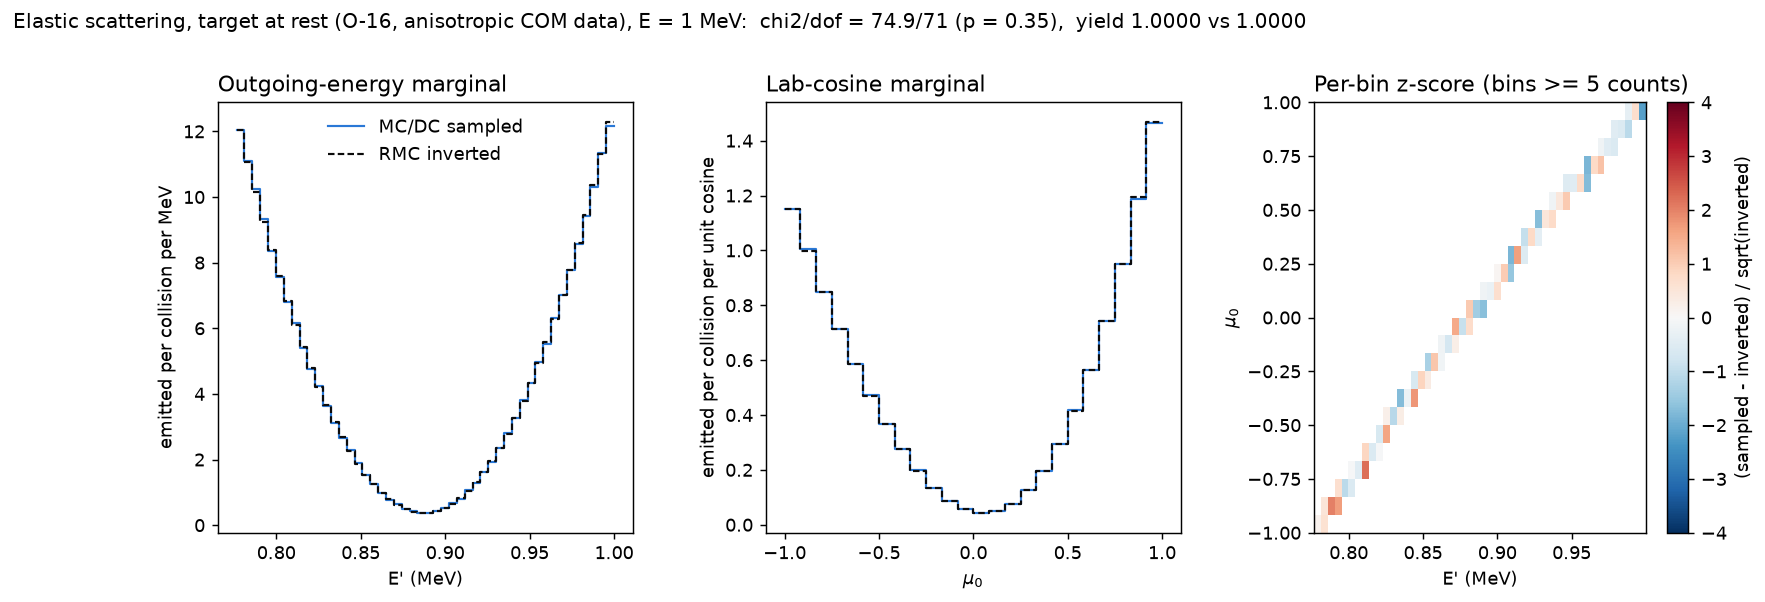
\includegraphics[width=\textwidth]{figures/elastic/elastic_E1e06.png}
  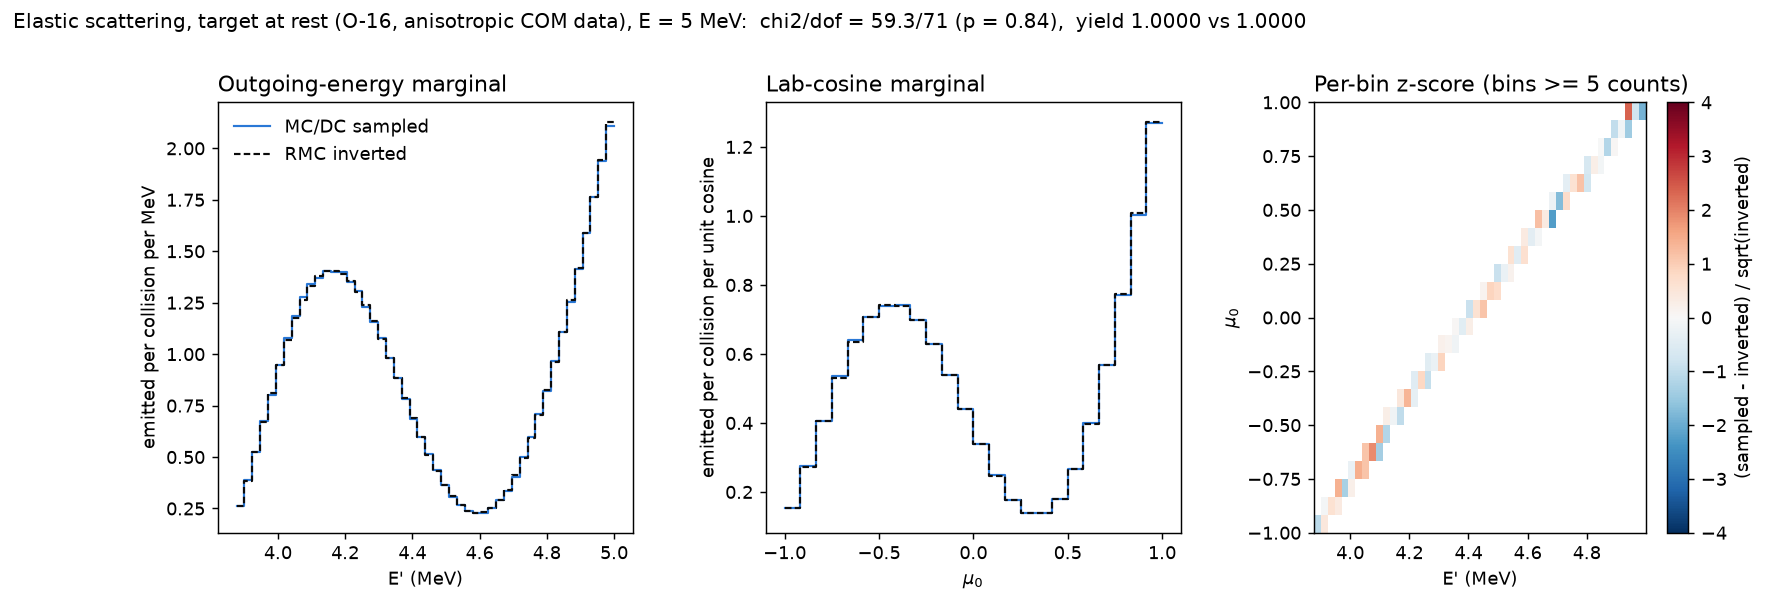
\includegraphics[width=\textwidth]{figures/elastic/elastic_E5e06.png}
  \caption{O-16 elastic scattering (ENDF/B-VIII.1, 293.6\,K, anisotropic COM
  data) at 1 and 5\,MeV. The line kernel occupies one cosine bin per energy bin.}
\end{figure}

\end{document}
